\documentclass[a4paper, 11pt]{book}
% \usepackage{/home/nora/Documents/Enseignement/Prepa/bpep/fichiers_utiles/preambule}
\usepackage{cours-preambule}

\makeatletter
\renewcommand{\@chapapp}{Kh\^olles MPSI -- semaine}
\makeatother
\renewcommand\thechapter{18}

% \toggletrue{student}
% \toggletrue{corrige}

\begin{document}

\settype{enon}
\settype{solu}

\chapter{Sujet 1\siCorrige{\!\!-- corrig\'e}}
\resetQ
\subimport{/home/nora/Documents/Enseignement/Prepa/bpep/exercices/TD/oscilloscope_analogique/}{sujet.tex}

\chapter{Sujet 2\siCorrige{\!\!-- corrig\'e}}
\resetQ
\section{Pendule électrique}
\enonce{%
	On étudie un pendule constitué d'une boule de polystyrène expansé recouverte
	d'une feuille d'aluminium, et suspendue à une potence par une fine tige de
	longueur $R = \SI{10}{cm}$ dont nous négligerons la masse. La boule de masse
	$m = \SI{20}{g}$ sera assimilée à un point matériel M.
	\smallbreak
	Une boule identique est placée en A (voir schéma). Les deux boules sont
	chargées électriquement avec la même charge, et donc se repoussent. La force
	exercée par A sur M s'écrit
	\[
		\Ff_e = \frac{k}{\rm AM^3} \vv{\rm AM}
		\qavec
		k = \SI{4.4e-3}{N.m^2}
	\]
	\bigbreak
	\noindent
	\begin{minipage}{0.45\linewidth}
		\begin{center}
			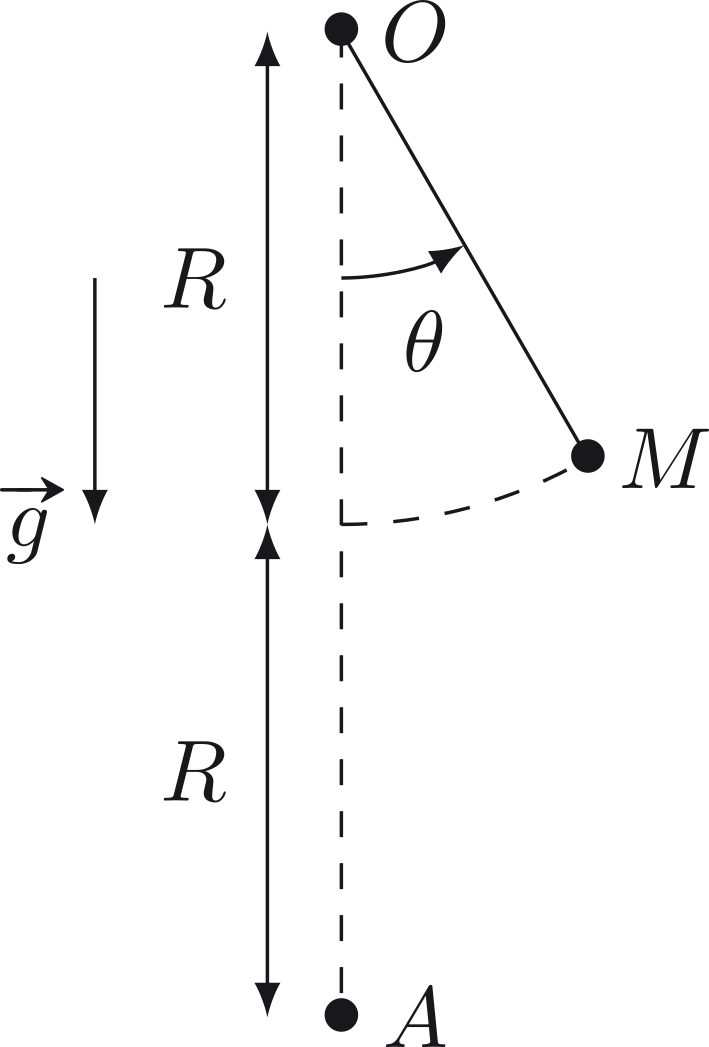
\includegraphics[height=4cm]{../figures/pendule_elec_sch-plain.png}
			\captionof{figure}{Dispositif}
		\end{center}
	\end{minipage}
	\hfill
	\begin{minipage}{0.35\linewidth}
		\begin{center}
			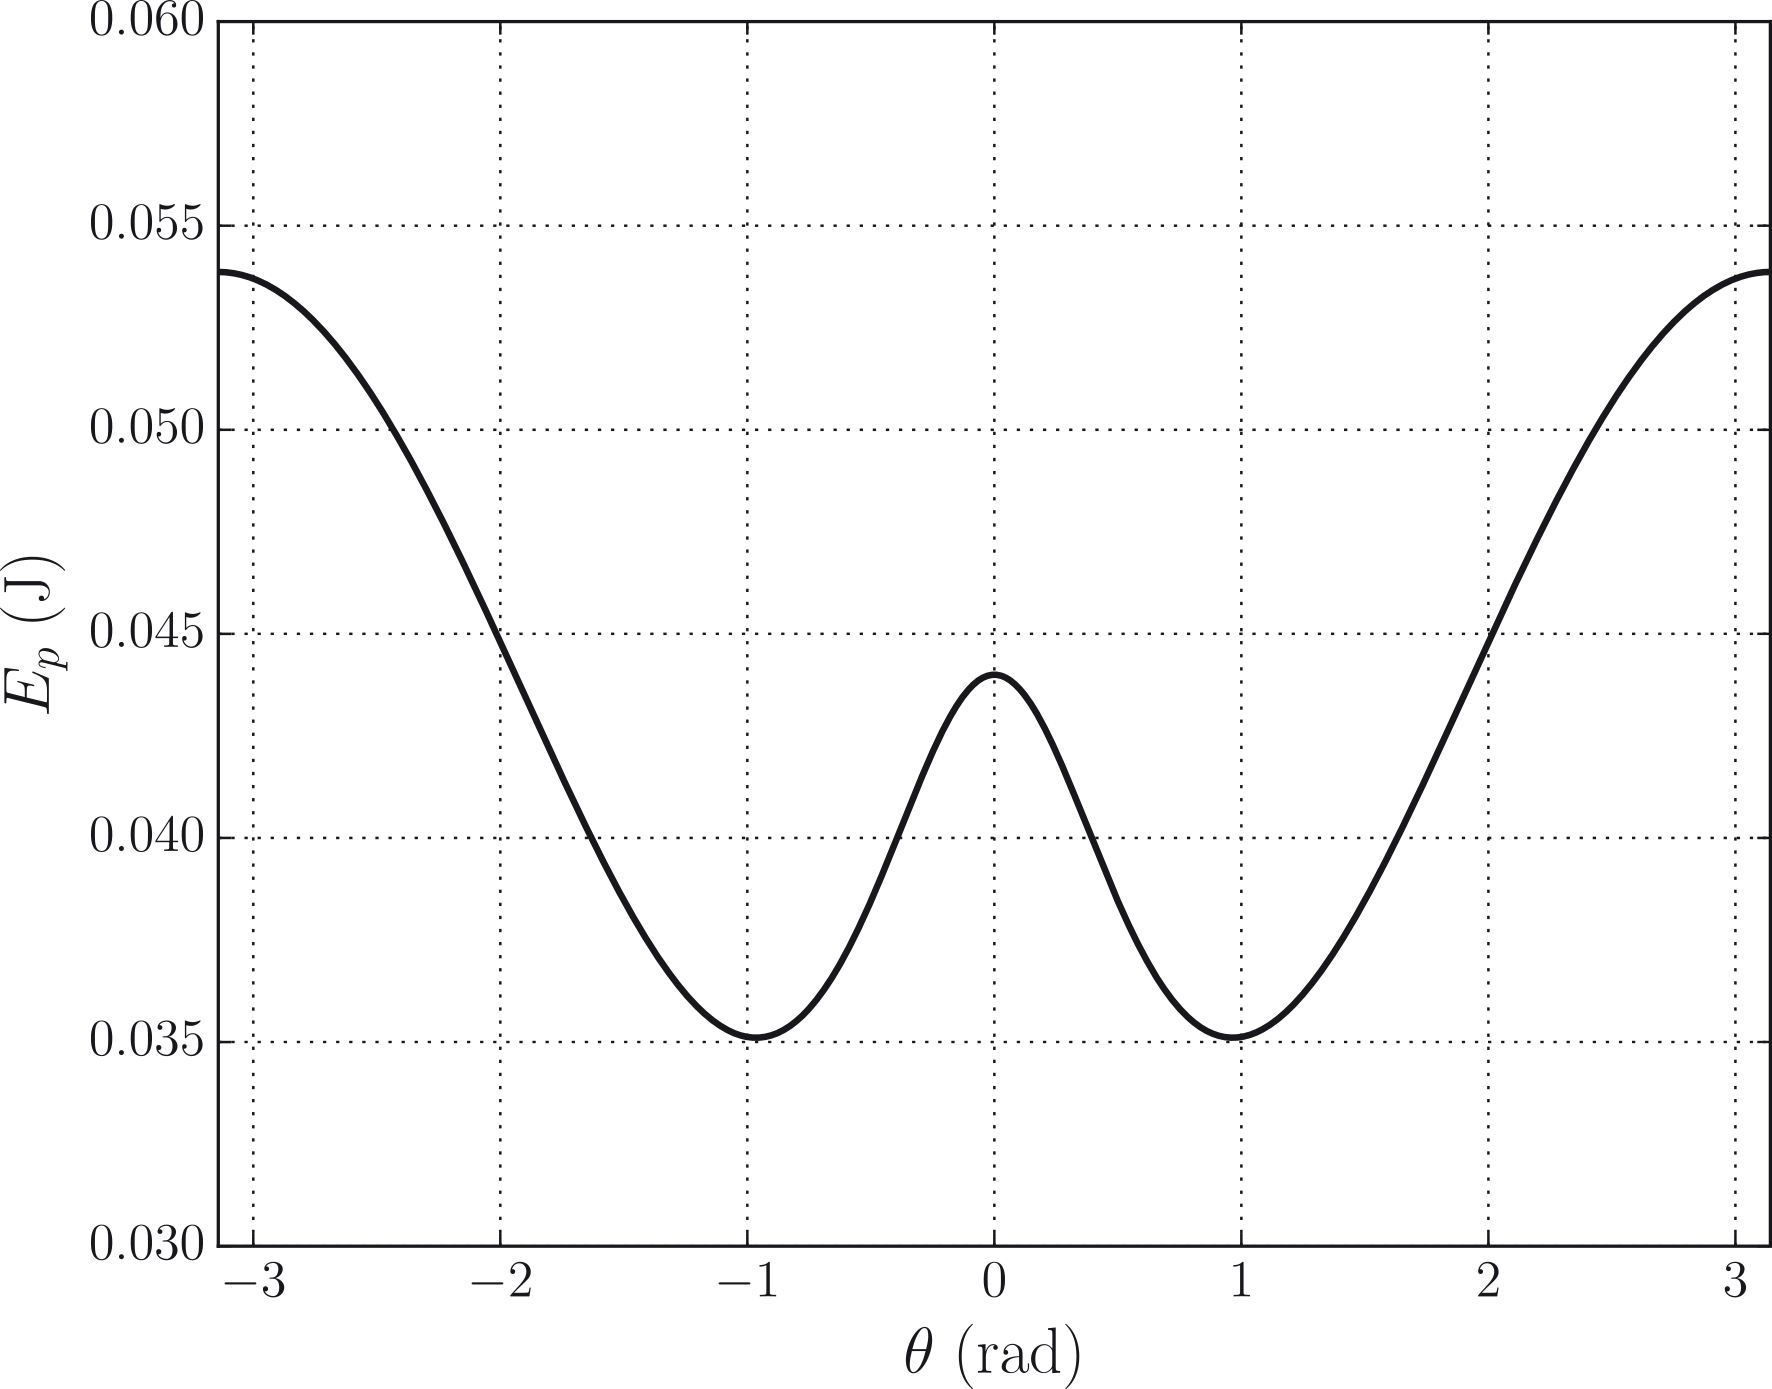
\includegraphics[width=\linewidth]{../figures/pendule_elec_ep-plain}
			\captionof{figure}{Courbe $\Ec_p(\th)$}
		\end{center}
	\end{minipage}
}
\QR{%
	Exprimer la distance AM en fonction de $R$ et $\th$.
}{%
	Pour exprimer la distance AM, on la décompose par des vecteurs connus
	et on pourra prendre la norme du vecteur $\vv{\rm AM}$ avec
	$\sqrt{x_{\rm AM}{}^2 + y_{\rm AM}{}^2}$, ou $\sqrt{\vv{\rm
				AM}\cdot\vv{\rm AM}}$. Notamment, $\vv{\rm AM} = \vv{\rm AO} + \OM$.

	\begin{minipage}[t]{0.33\linewidth}
		~%\vspace{-24pt}
		\begin{center}
			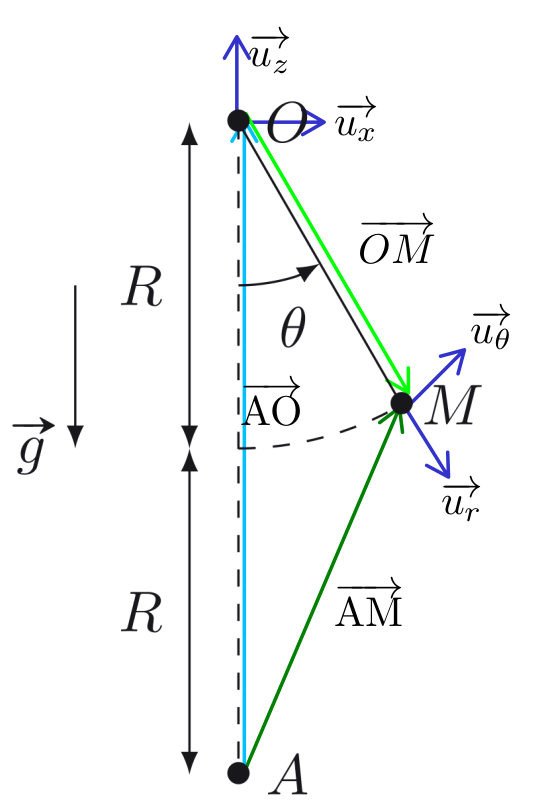
\includegraphics[width=.8\linewidth]{../figures/pendule_elec_am}
			\captionsetup{justification=centering}
			\captionof{figure}{Détermination de AM}
			\label{fig:pendule_am}
		\end{center}
	\end{minipage}
	\hfill
	\begin{minipage}[t]{0.65\linewidth}
		Il faut donc décomposer $\vv{\rm AO}$ et $\OM$ sur la même base,
		comme on le fait pour le poids sur un plan incliné. En effet,
		\begin{align*}
			\vv{\rm AO} = 2R\uz
			\qet
			\OM         = R\ur
		\end{align*}
		mais on ne peut pas sommer les deux dans des bases différentes.
		Décomposons $\ur$ sur $(\ux, \uz)$~: on trouve
		$\ur = \sin\th\ux -\cos\th\uz$
		Ainsi,\vspace{-24pt}
		\begin{align*}
			\vv{\rm AM}        & = \vv{\rm AO} + \OM
			\\\Lra
			\vv{\rm AM}        & = \mqty(R\sin\th                                        \\2R-R\cos\th)
			\\\Ra
			\norm{\vv{\rm AM}} & = \sqrt{R^2\sin^2\th + (2R-R\cos\th)^2}
			\\\Lra
			{\rm AM}           & = \sqrt{R^2\sin^2\th + 4R^2 -2R^2\cos\th +R^2\cos^2\th}
			\\\Lra
			{\rm AM}           & = \sqrt{5R^2 -2R^2\cos\th}
			\qavec
			\cos^2\th + \sin^2\th = 1
			\\\Lra
			\Aboxed{{\rm AM}   & = R\sqrt{5-2\cos\th}}
			\qed
		\end{align*}
	\end{minipage}
}
\QR{%
	Montrer que la force $\Ff_e$ est conservative, et que son énergie
	potentielle s'exprime
	\[\Ec_{p,e}(\th) = \frac{k}{R\sqrt{5-4\cos\th}}\]
}{%
	Une force est conservative si son travail élémentaire s'exprime sous
	la forme $-\dd\Ec_p$. Calculons son travail élémentaire~:
	\begin{align*}
		\de W(\Ff_e)         & = \Ff_e\cdot\dd{\vv{\rm AM}}
		\\\Lra
		\de W(\Ff_e)         & = \frac{k}{\rm AM^3}{\vv{\rm AM}}\cdot\dd{\vv{\rm AM}}
		\\\Lra
		\de W(\Ff_e)         & = \frac{k}{\rm AM^3} \underbracket[1pt]{\norm{\vv{\rm
					AM}}}_{=\rm AM} \norm{\dd{\vv{\rm AM}}}
		\underbracket[1pt]{\cos(\vv{\rm AM}, \dd{\vv{\rm AM}})}_{=1}
		\\\Lra
		\de W(\Ff_e)         & = \frac{k}{\rm AM^2} \cancel{\underbracket[1pt]{\frac{\rm
					AM}{\rm AM}}_{=1}} \dd{\rm AM}
		\\\Lra
		\de W(\Ff_e)         & = -k\dd(\frac{1}{\rm AM})
		\\\Lra
		\Aboxed{\de W(\Ff_e) & = -\dd{\Ec_{p,e}}}
		\\\qavec
		\Aboxed{\Ec_{p,e}    & = \frac{k}{\rm AM} = \frac{k}{R\sqrt{5-4\cos\th}}}
		\qed
	\end{align*}
}
\QR{%
	Exprimer l'énergie potentielle totale $\Ec_p(\th)$ de la boule M.
}{%
	La boule M a également une énergie potentielle de pesanteur. En
	prenant O comme origine de l'altitude, l'altitude de la boule M $z(\th)$
	s'exprime
	\[z(\th) = -R\cos\th\]
	Ainsi,
	\begin{align*}
		\Ec_p(\th)         & = \Ec_{p,p}(\th) + \Ec_{p,e}(\th)
		\\\Lra
		\Aboxed{\Ec_p(\th) & = \frac{k}{R\sqrt{5-4\cos\th}} - mgR\cos\th}
		\qed
	\end{align*}
}
\QR{%
	Le tracé de l'énergie potentielle est proposé sur la figure 2. Déduire
	de ce graphe l'existence de positions d'équilibres, et indiquer leur
	nature.
}{%
	On observe en tout 5 positions d'équilibres~: deux stables dans les
	puits de potentiel vers $\pm\SI{1}{rad}$, et trois instables (maxima
	locaux d'énergie potentielle) en $-\pi$, $0$ et $\pi$.
}
\QR{%
	Discuter de la nature de la trajectoire de M suivant la valeur de son
	énergie mécanique.
}{%
	Le mouvement du pendule ne se fait que dans les zones du graphique où
	$\Ec_p < \Ec_m$. On distingue donc 4 cas~:
	\[
		\begin{array}{lrcll}
			\textbf{Cas 1} & \quad \SI{0}{J}      & < \Ec_m & < \SI{3.5e-2}{J} & \Ra
			\text{pas de mouvement}
			\\
			\textbf{Cas 2} & \quad \SI{3.5e-2}{J} & < \Ec_m & < \SI{4.4e-2}{J} & \Ra
			\text{oscillations $\approx$ position stable}
			\\
			\textbf{Cas 3} & \quad \SI{4.4e-2}{J} & < \Ec_m & < \SI{5.4e-2}{J} & \Ra
			\text{mouvement périodique entre $\Ec_{p,\max}$}
			\\
			\textbf{Cas 4} & \quad \SI{5.4e-2}{J} & < \Ec_m & < +\infty        & \Ra
			\text{mouvement révolutif~: tours à l'infini}
		\end{array}
	\]
	\begin{center}
		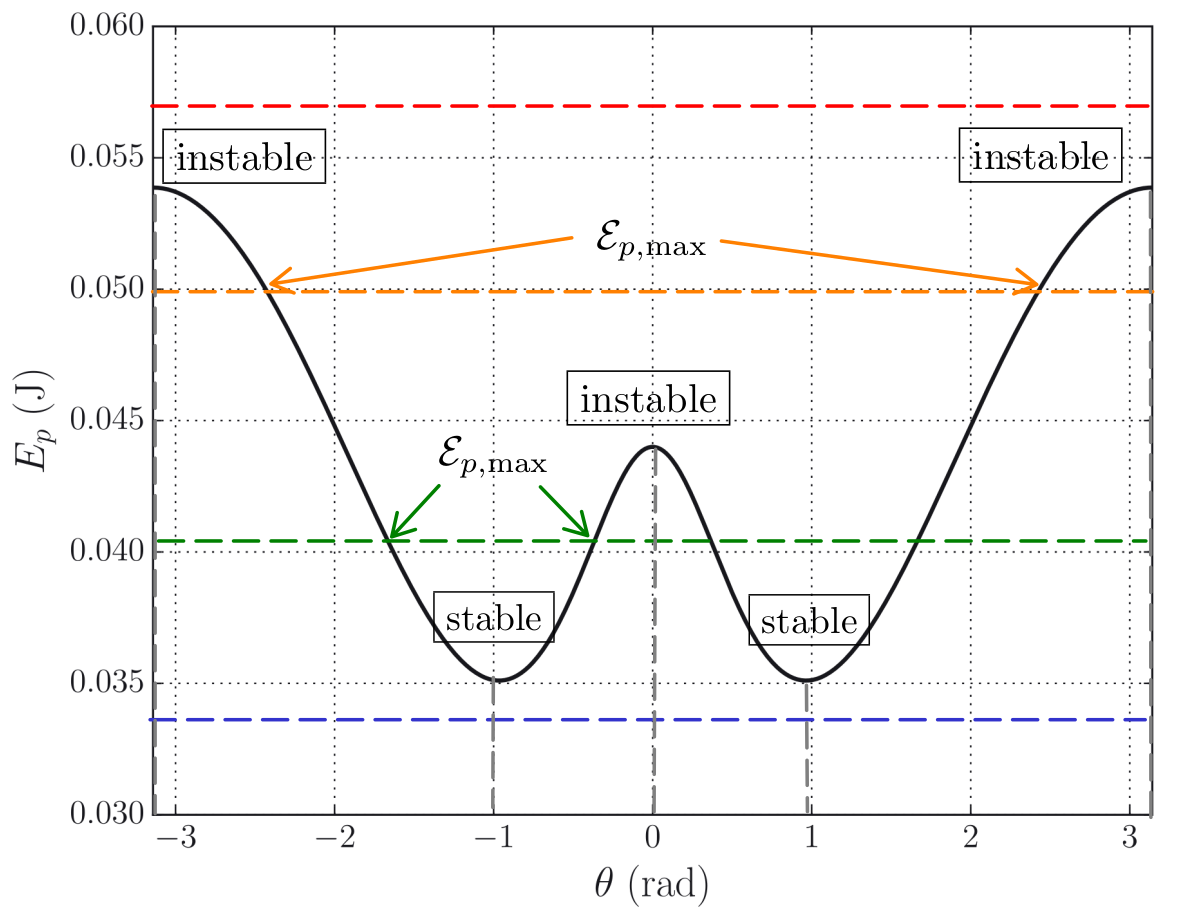
\includegraphics[width=.7\linewidth]{../figures/pendule_elec_ep_corr}
		\captionof{figure}{Mouvement selon $\Ec_m$}
		\label{fig:pend_elec_em}
	\end{center}
}

\chapter{Sujet 3\siCorrige{\!\!-- corrig\'e}}

\resetQ
\subimport{/home/nora/Documents/Enseignement/Prepa/bpep/exercices/Colle/champ_magnetique_et_frottements_fluides/}{sujet.tex}

\label{LastPage}
\end{document}
